\section{Moderne Festkörpertheorie}

\subsection{Energiebänder}
\begin{minipage}{0.5\linewidth}
	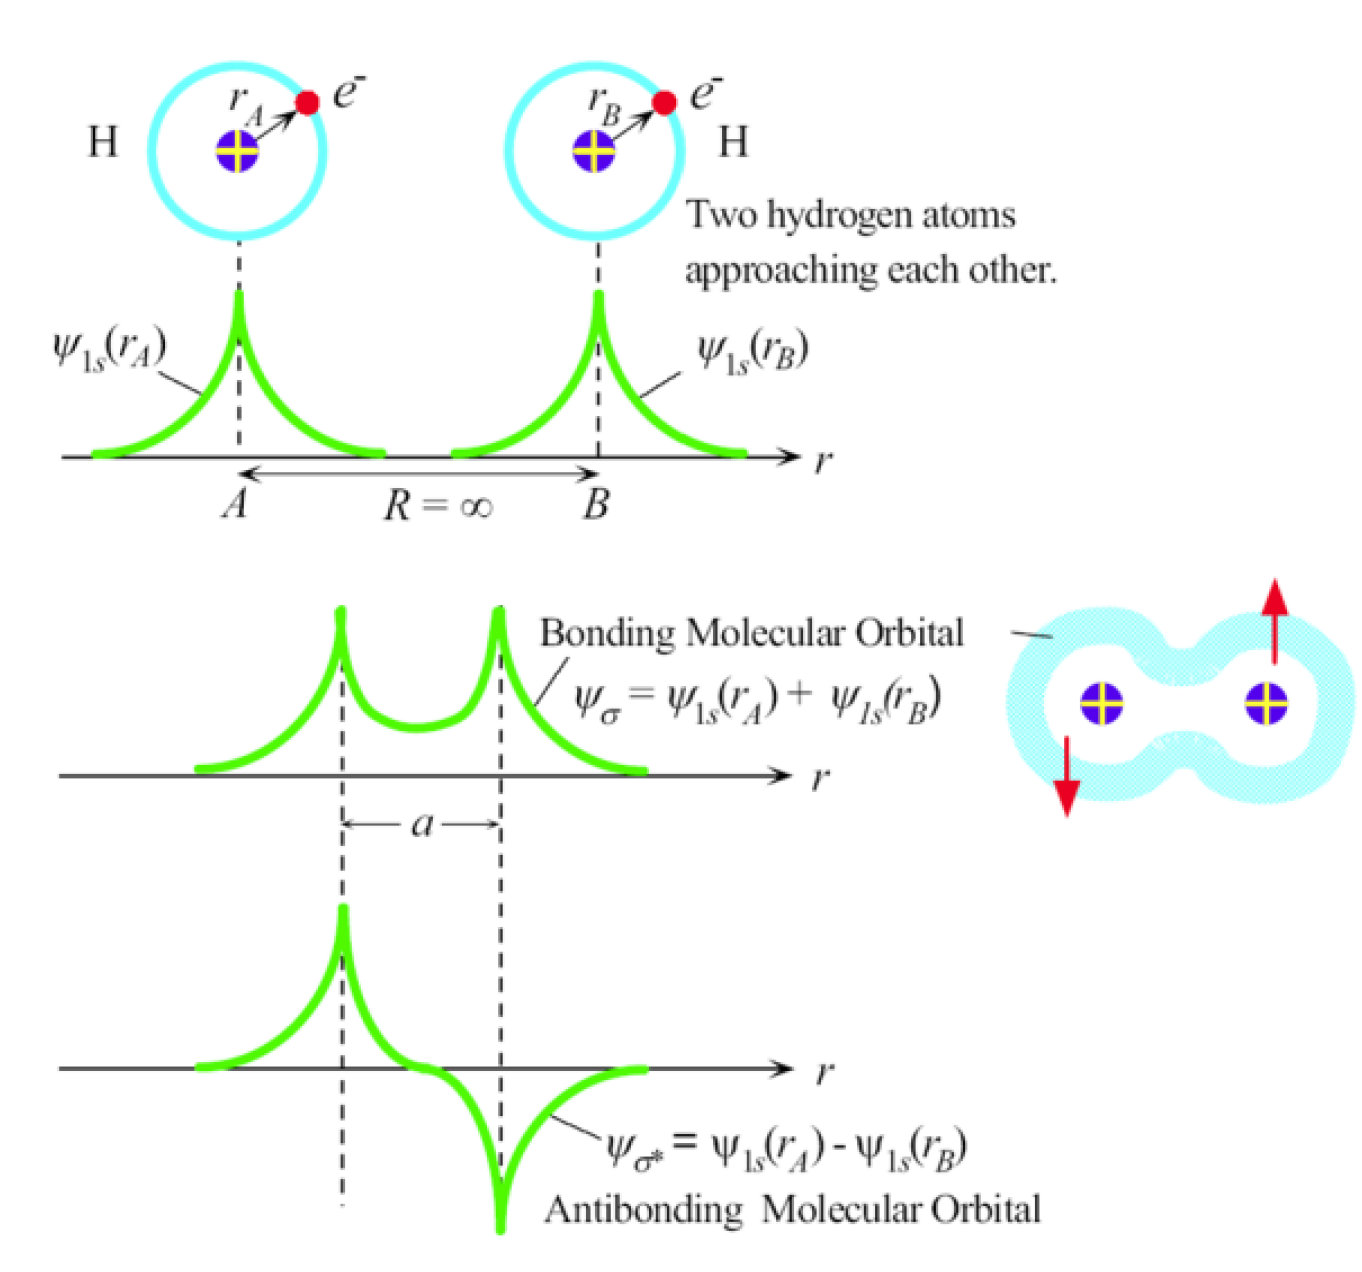
\includegraphics[width=0.99\linewidth]{Bilder/LCAO}
\end{minipage}
\hfill
\begin{minipage}{0.45\linewidth}
	\begin{itemize}
		\item Wellenfunktionen mehrerer Atome (hier 2) können symmetrisch oder antisymmetrisch kombiniert werden. 
		\item Die neu entstandenen Orbitale nennt man Molekülorbitale 
		\item $\Rightarrow$ LCAO(linear comb. of atomic orbitals)
		\item Il numero di \textit{nodi} (intersezioni con l'asse $x$) di $\Psi$ indica il livello
		di Energia (+ nodi $= + E$)
	\end{itemize}\vspace{0.5em}
	
	${\Psi }_{\sigma }=\Psi \left({r}_{a}\right)+\Psi \left({r}_{b}\right)$

	${\Psi^*}_{\sigma }=\Psi \left({r}_{a}\right)-\Psi \left({r}_{b}\right)$
\end{minipage}

\subsubsection{Energiebänder von Metallen}
Die Energie, bis zu welcher das Band besetzt ist, wird Fermi-Energie genannt. 

(Li-Ionen-Kette)

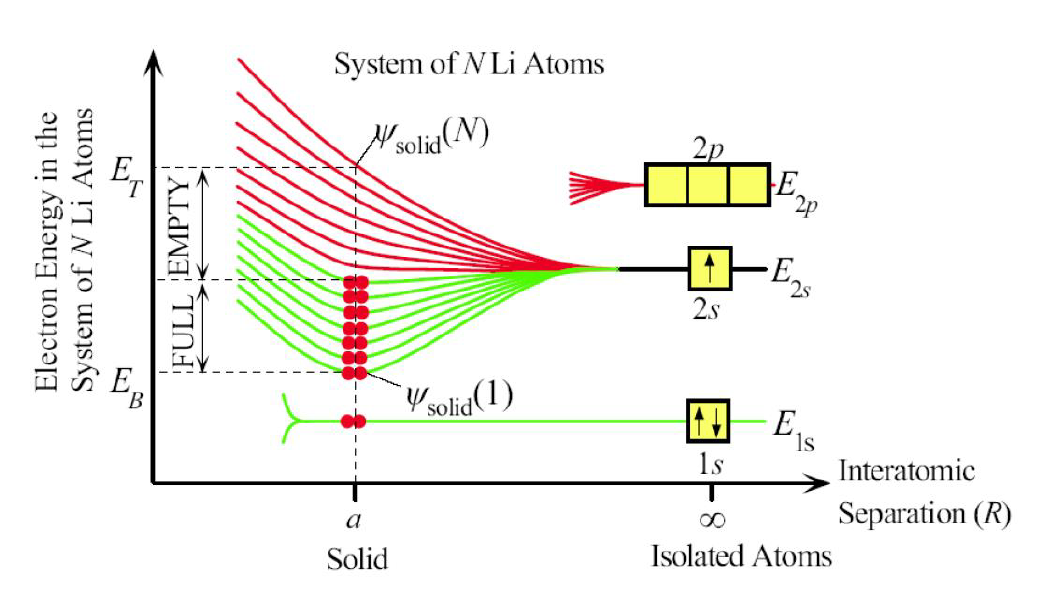
\includegraphics[width=0.85\linewidth]{Bilder/Energieband_Li}

\begin{minipage}{0.6\linewidth}
	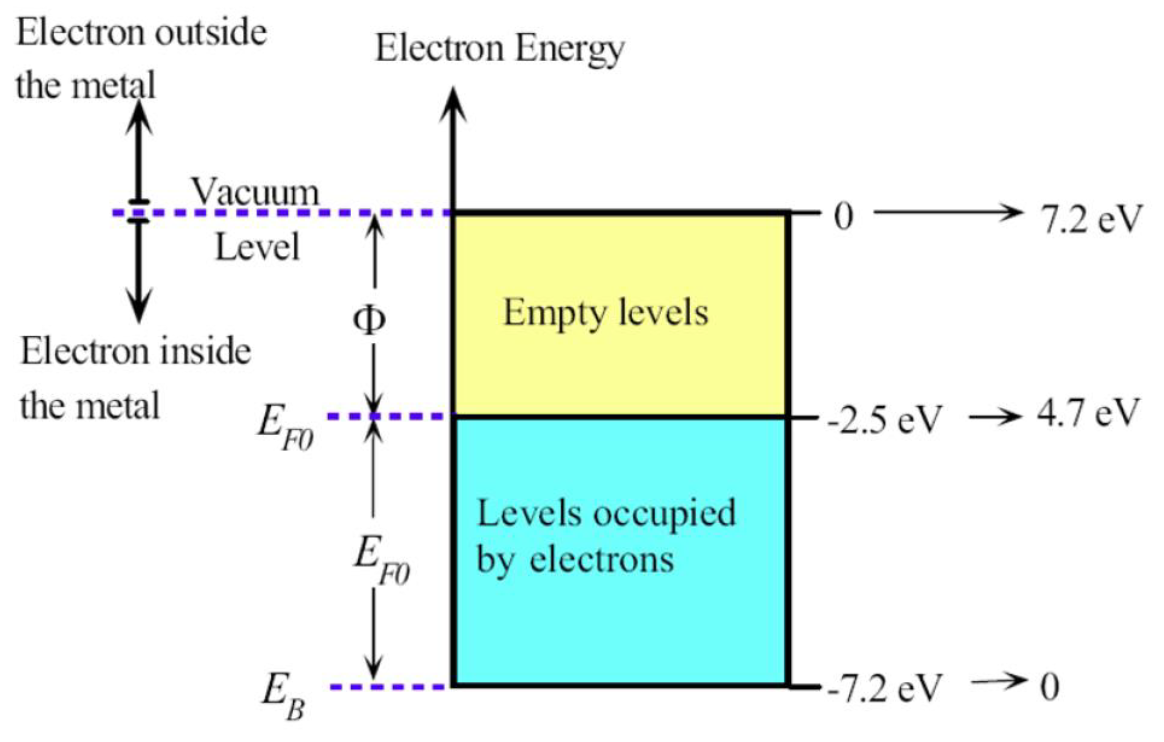
\includegraphics[width=0.99\linewidth]{Bilder/Elektron-Energieband}
\end{minipage}
\hfill
\begin{minipage}{0.4\linewidth}
	\begin{itemize}
		\item Das ist ein typisches Elektron-Energieband eines Metalls.
		\item Die Valenzelektronen füllen das Band \cor{von unten nach oben auf.}
		\item Die Grenze zwischen \textit{besetzten} und \textit{leeren} Zuständen wird \textbf{Fermi-Energie} $E_{F0}$ genannt.
		\item Im \textbf{Vakuum}-Zustand sind die Elektronen nicht mehr gebunden, somit besitzen sie keine negative potentielle Energie mehr.
	\end{itemize}
\end{minipage}

\subsection{Bänder-Modell im Impulsraum}

	\begin{minipage}{0.5\linewidth}
		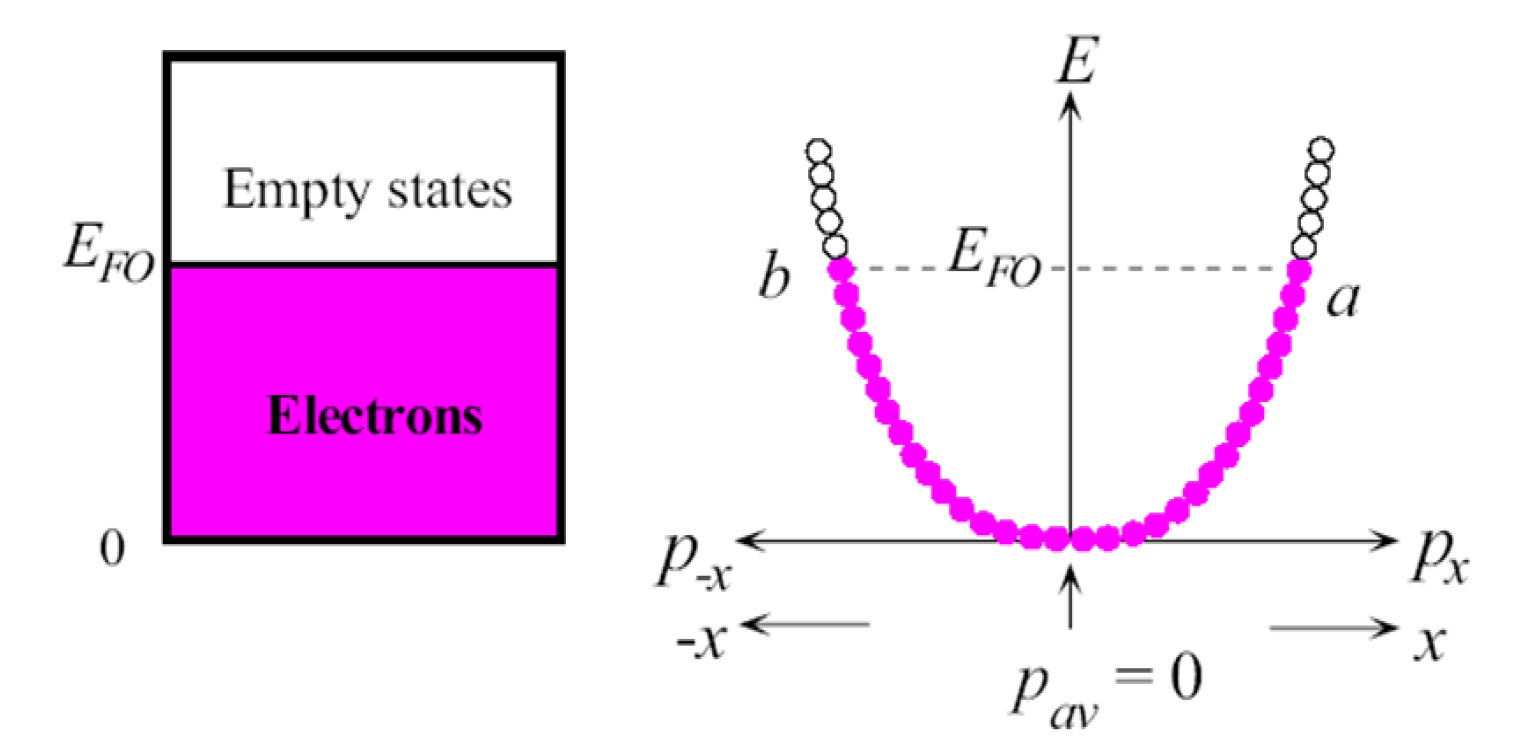
\includegraphics[width=0.99\linewidth]{Bilder/Modell_1}
	\end{minipage}
	\hfill
	\begin{minipage}{0.5\linewidth}
		Bewegte Teilchen haben immer auch einen Impuls, d.h man kann das Bändermodell auch im Impulsraum betrachten. 
		Durch lösen der Schrödingergleichung erhält man für die Energie des Elektrons:

		\[E=\frac{\hbar^2 k^2}{2m}=\frac{p^2}{2m}\]

		Somit sieht das Energieband wie eine Parabel aus.
	\end{minipage}
	\vspace{2mm}

	Die \textbf{elektrische Leitfähigkeit} kann ebenfalls am Bandmodell erklärt werden. 
	Durch Anlegen einer Spannung kippt die Fermi-Fläche, was dazu führt, 
	dass sich die Impulse nicht mehr kompensieren und ein Strom fliesst. 
	Das ist im Ortsraum auch so, wobei sich dort die Energiezustände verkippen.

	\begin{minipage}{0.48\linewidth}
		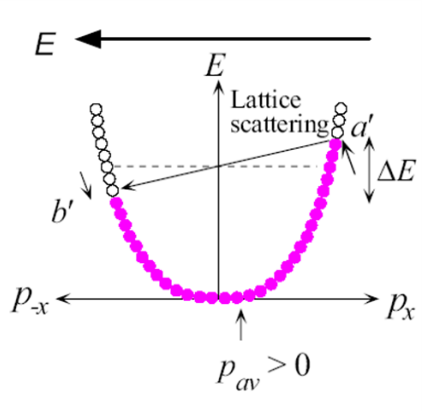
\includegraphics[width=0.99\linewidth]{Bilder/Modell_2}
	\end{minipage}
	\hfill
	\begin{minipage}{0.48\linewidth}
		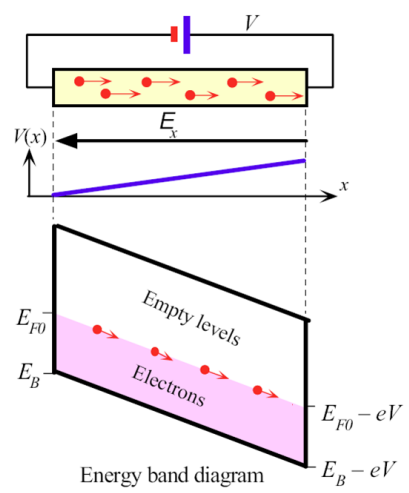
\includegraphics[width=0.99\linewidth]{Bilder/Modell_3}
	\end{minipage}

\subsection{Bänder-Modell für Halbleiter und Isolatoren}

2 Si-Atome mit LCAO-Methode $\Rightarrow$ 1 volles Valenzband \& 1 leeres Leitungsband

\begin{itemize}
	\item Dazwischen liegt Bandlücke $\rightarrow$ Fermi-Fläche $E_g$ (posti liberi stadio)
	\item Anlegen von Spannung hat \textbf{keinen Strom} zur Folge, ausser ...
	\begin{itemize}
		\item Spannung müsste gross genug sein, um isol. Zustand zu brechen, oder ...
		\item thermisch aktivierte Elektronen im Leitungsband
	\end{itemize}
\end{itemize}

\begin{minipage}{0.6\columnwidth}
	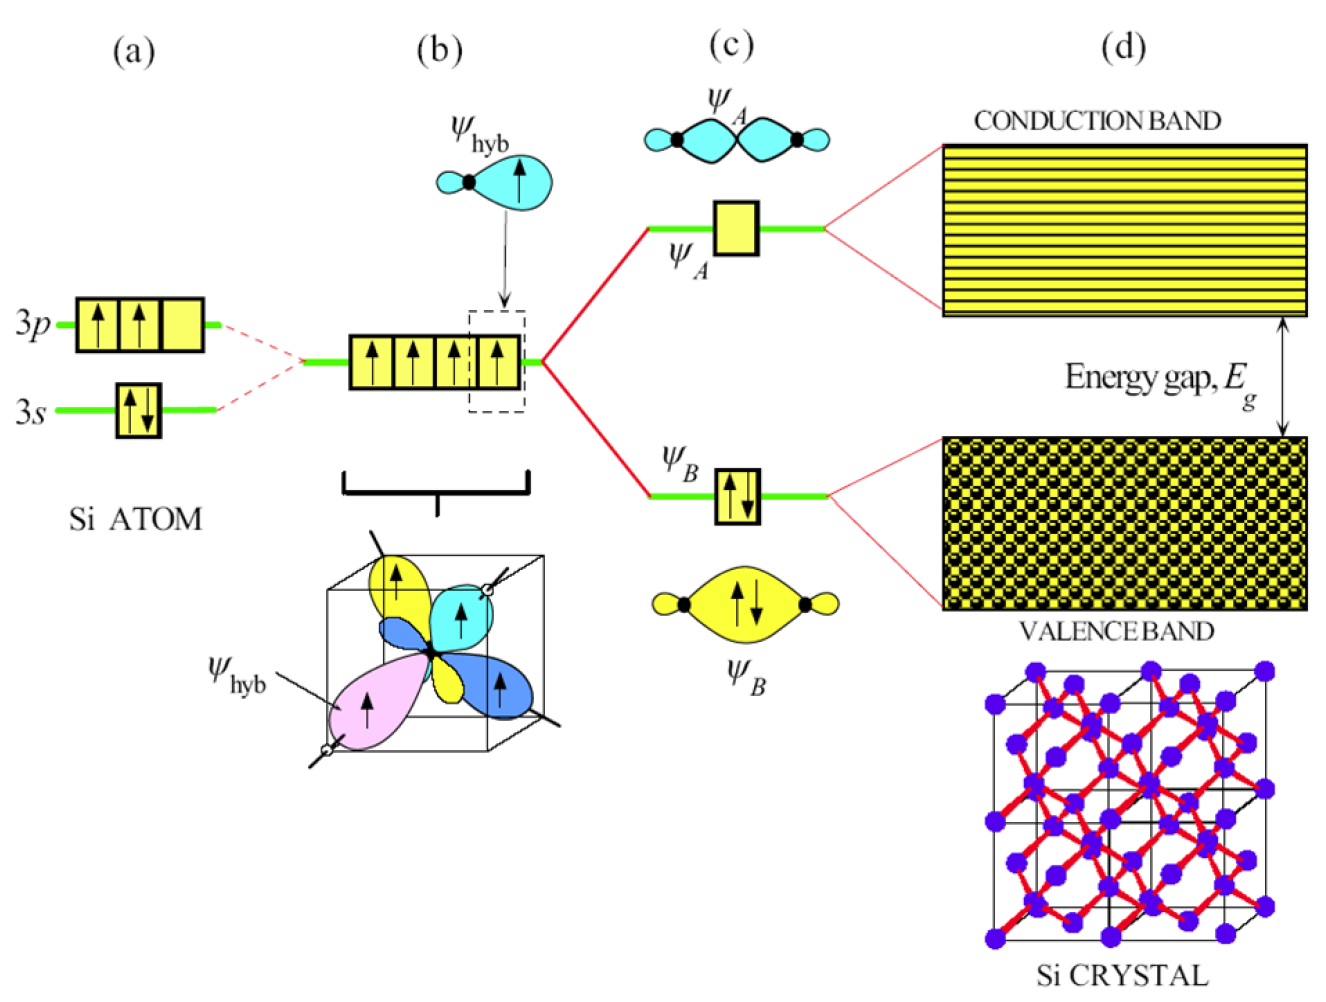
\includegraphics[width=0.99\linewidth]{Bilder/Bandstruktur_Si}
\end{minipage}
\hfill
\begin{minipage}{0.15\columnwidth}
	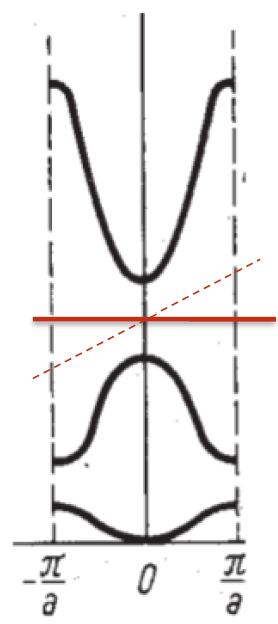
\includegraphics[width=0.8\linewidth]{Bilder/Bandstruktur_Si_2}
\end{minipage}
\hfill
\begin{minipage}{0.2\columnwidth}
	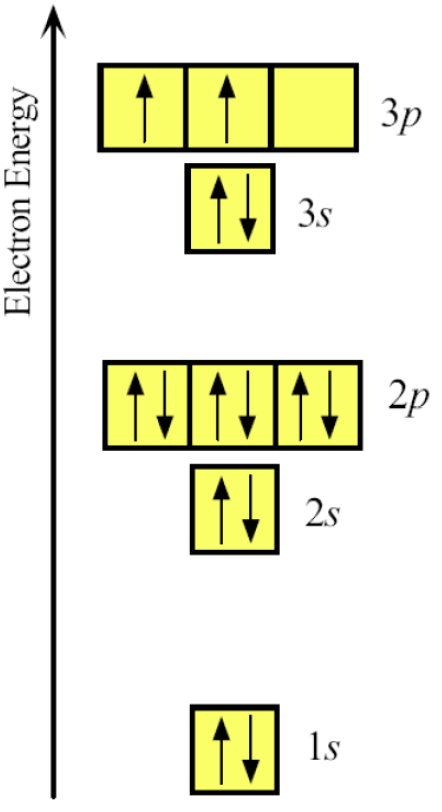
\includegraphics[width=0.85\linewidth]{Bilder/Bandstruktur_Si_3}
\end{minipage}

\subsection{Zustandsdichte in Energiebändern}

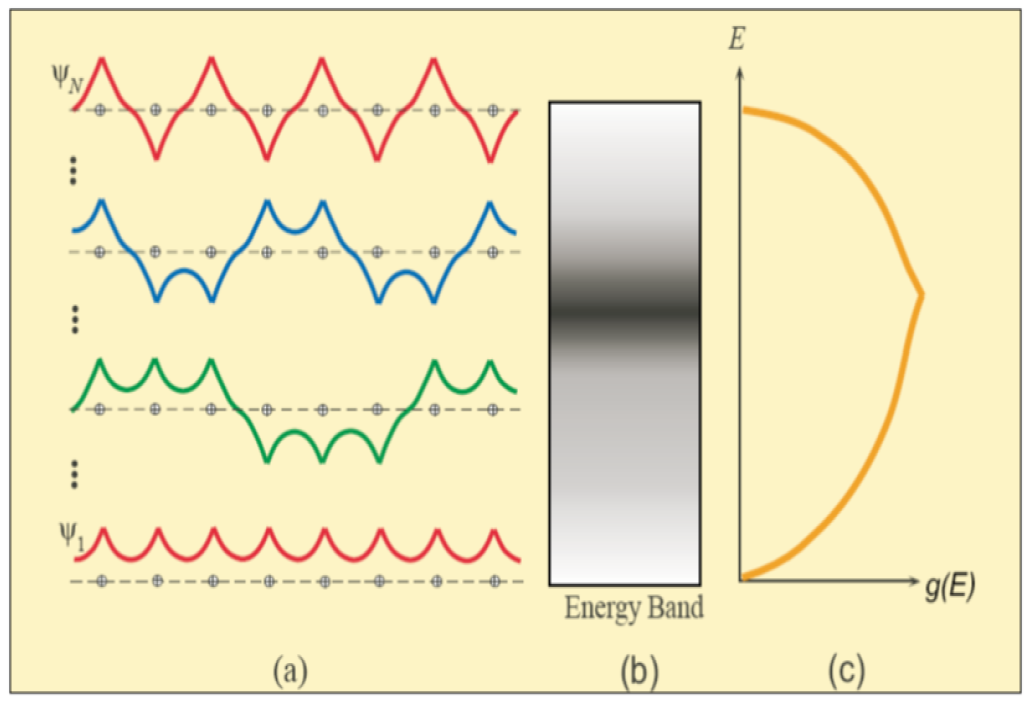
\includegraphics[width=0.9\linewidth]{Bilder/Zustandsdichte}

Man kann eine sogenannte Zustandsdichte \textbf{(c)} definieren, welche beschreibt, 
wie viele Zustände im Band für einen Energiebereich existieren (per i livelli energetici centrali
esistono diverse soluzioni di $\Psi$ con lo stesso numero di 'knoten'). (Im Bild N=8 atomi)

Die \textbf{Boltzmann-Energie-Verteilung} beschreibt die Statistik der Elektronen, 
solange deutlich mehr Zustände verfügbar sind als Elektronen, da dann Quantenmechanik eine untergeordnete Rolle spielt.

\subsection{Verteilungen}

Descrive la porbabilità di trovare elettroni ad uno specifico livello energetico\medskip

\begin{minipage}[t]{0.49\linewidth}
	\textbf{Meccanica classica}

	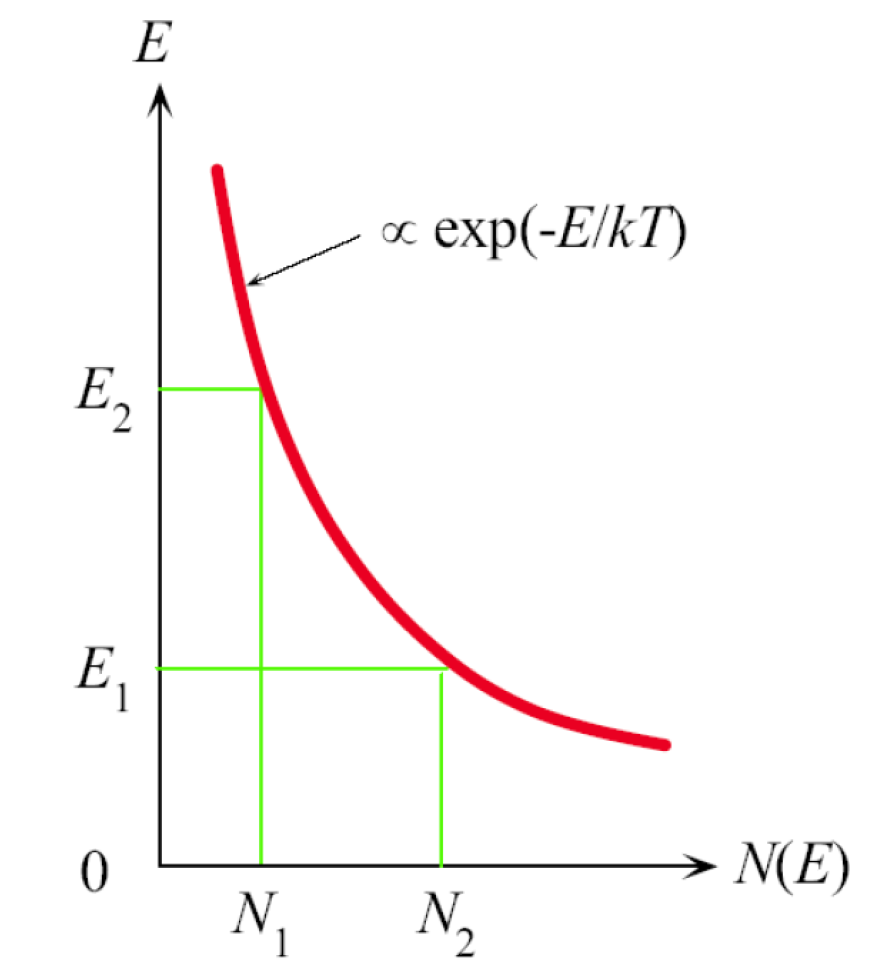
\includegraphics[width=0.7\linewidth]{Bilder/boltzmann-vert}

	\[ P (E) = A \cdot e^{-\frac{E}{k_BT}} \]
\end{minipage}
\hfill
\begin{minipage}[t]{0.5\linewidth}
	\textbf{Fisica quantistica} (pauli prinzip)
	
	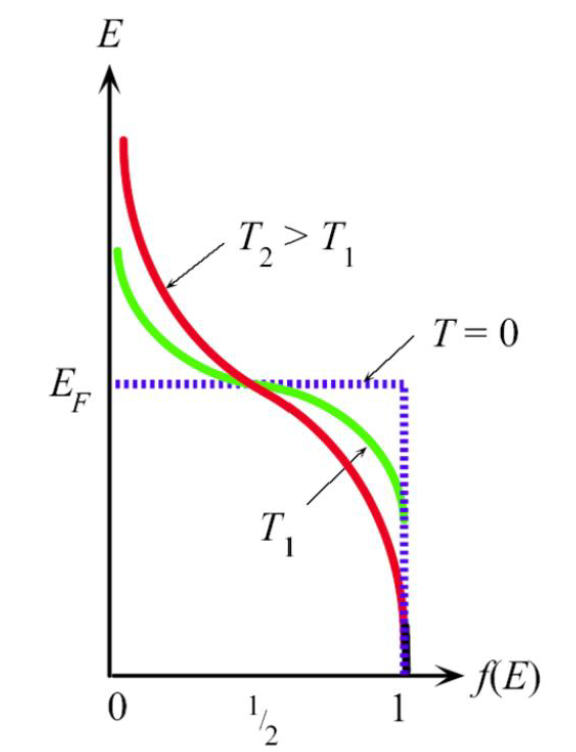
\includegraphics[width=0.7\linewidth]{Bilder/Fermi_Dirac}

	\[ P (E) = \dfrac{1}{1+A \cdot e^{\frac{E-E_F}{k_BT}}} \]
\end{minipage}

\subsubsection{Metall-Metall-Kontakt}

	\begin{minipage}{0.49\linewidth}
		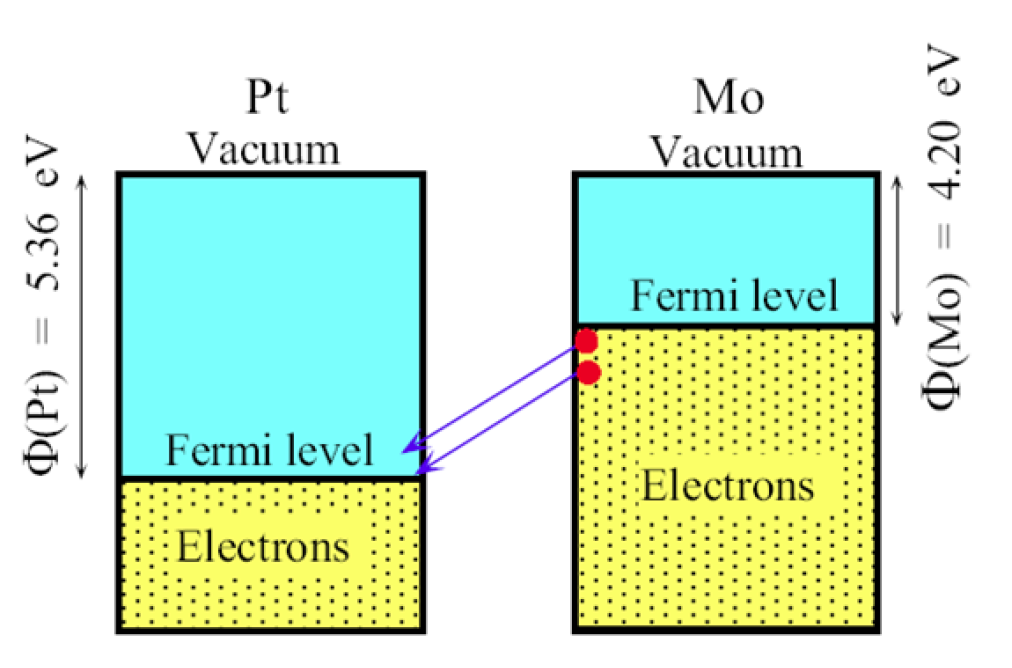
\includegraphics[width=0.99\linewidth]{Bilder/Fermi_Metall_1}
	\end{minipage}
	\begin{minipage}{0.5\linewidth}
		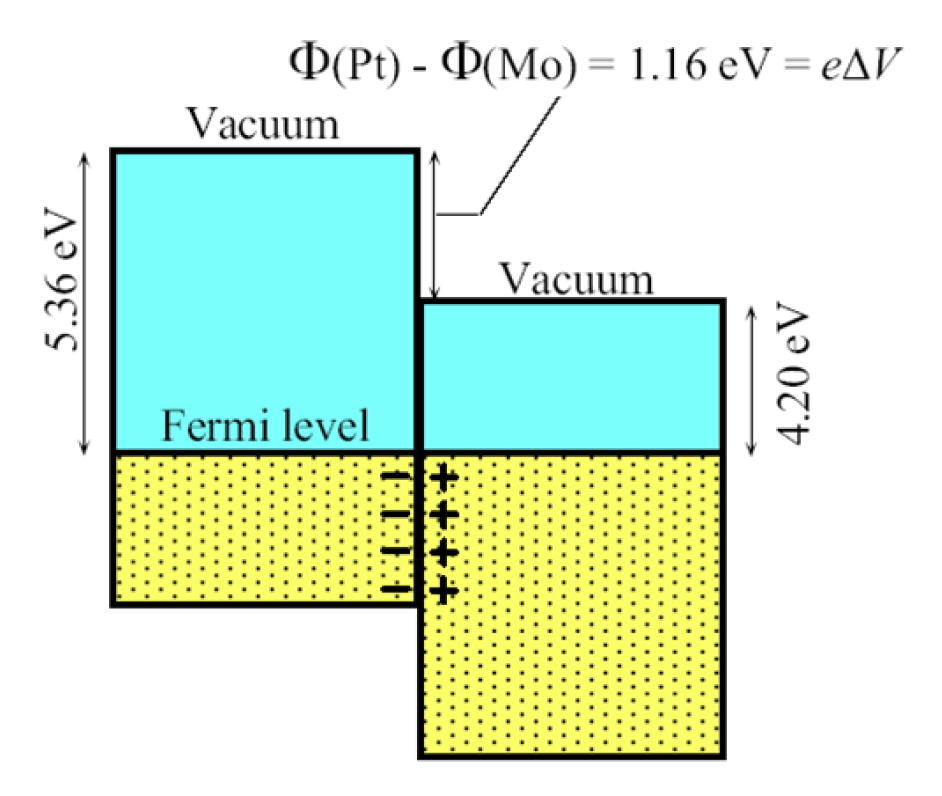
\includegraphics[width=0.99\linewidth]{Bilder/Fermi_Metall_2}
	\end{minipage}

Molybdän und Platin werden kontaktiert:
\begin{itemize}
	\item Fermi-Flächen passen sich an $\rightarrow$ Vakuumniveau verschiebt sich
	\item[$\Rightarrow$] Kontaktspannung = Differenz der Austrittsarbeiten
	\item[$\Rightarrow$] Kontaktspannung kann \textbf{keine} Arbeit verrichten
\end{itemize}

\subsubsection{Seebeck-Effekt}
\begin{minipage}{0.5\linewidth}
	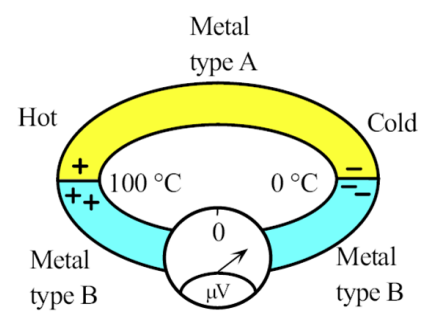
\includegraphics[width=0.99\linewidth]{Bilder/Seebeck_Effekt}
\end{minipage}
\begin{minipage}{0.5\linewidth}
	Mit dem Seebeck-Effekt lassen sich Thermoelemente realisieren. 
	Zwei Metalle mit unterschiedlichem Seebeck-Koeffizient werden kombiniert. 
	Die Kontaktstellen werden unterschiedlichen Temperaturen ausgesetzt. 
	Mittels Spannungsmessung kann der Temperaturunterschied gemessen werden.
\end{minipage}